% ============================================================
% SUPPLEMENTARY MATERIAL
% Optical Profilometry Versus the Stylus:
% A Spectral Theory for Closing the Accuracy Gap
% ============================================================
\documentclass[review,12pt]{elsarticle}

\usepackage{amsmath,amssymb}
\usepackage{graphicx}
\usepackage{booktabs}
\usepackage{hyperref}
\usepackage{lineno}
\usepackage{siunitx}

\begin{document}

\title{Supplementary Material: Physical Framework, Scatterometry Extension, and Surface-Class Stress-Test}

\author[1]{Dawid Kucharski}
\affiliation[1]{organization={Institute of Mechanical Engineering},
              addressline={Poznan University of Technology},
              city={Pozna\'{n}},
              postcode={60-965},
              country={Poland}}

\maketitle

\linenumbers


\section{Complete Physical Framework: From Contact Mechanics to Vector Diffraction}
\label{sec:physics}
% ============================================================

The operator-theoretic and information-theoretic frameworks of the main text (Methods and Information-Theoretic Analysis, Sections~2 and~5) treat the measurement as a mathematical operator $\mathcal{M}$ characterised by a transfer function $H(\mathbf{f})$ and noise PSD $S_\eta(\mathbf{f})$. However, in a real measurement, $H(\mathbf{f})$ and $S_\eta(\mathbf{f})$ are not arbitrary---they emerge from underlying physical processes that differ fundamentally between tactile (stylus) and optical modalities. This section completes the physical picture by incorporating the governing physics of both measurement principles.

\subsection{Hertzian Contact Mechanics of Stylus Profilometry}

A diamond stylus with tip radius $r_\mathrm{tip} = \SI{2}{\micro m}$ under a normal load of $F_n = \SI{1}{mN}$ contacts a steel surface ($E \approx \SI{200}{GPa}$, $H \approx \SI{5}{GPa}$). The Hertzian elastic contact theory~\cite{johnson1985contact} predicts a circular contact area of radius:
\begin{equation}
    a = \left(\frac{3 R_\mathrm{eff} F_n}{4 E_\mathrm{eff}}\right)^{1/3}
    \label{eq:hertz}
\end{equation}
where $1/E_\mathrm{eff} = (1-\nu_\mathrm{tip}^2)/E_\mathrm{tip} + (1-\nu_\mathrm{surf}^2)/E_\mathrm{surf}$. For the baseline parameters, the contact radius is $a = \SI{201}{nm}$, with a mean contact pressure $p_\mathrm{mean} = \SI{7.9}{GPa}$ and peak pressure $p_\mathrm{max} = \SI{11.8}{GPa}$.

The peak pressure exceeds the steel hardness ($H = \SI{5}{GPa}$), placing the contact in the \textbf{plastic regime}. The Greenwood--Williamson plasticity index~\cite{greenwood1966contact} is $\psi = (E_\mathrm{eff}/H)\sqrt{\sigma/r_\mathrm{tip}} = 5.83$, confirming significant plastic deformation. Two implications follow for stylus measurements:
\begin{enumerate}
    \item The Hertzian elastic analysis is not quantitatively valid in the plastic regime; the elastic contact radius $a \approx \SI{201}{nm}$ is retained only as an order-of-magnitude scale of the deformed zone. A quantitative prediction of the permanent groove depth would require an elastic--plastic contact model, which is beyond the scope of this work.
    \item For softer materials (aluminium, polymers), plastic deformation dominates and the stylus measurement becomes inherently destructive---the measured profile is the plastically deformed surface, not the original.
\end{enumerate}
The JKR adhesion correction~\cite{johnson1971surface} increases the effective contact radius by only \SI{1.5}{\percent} for the baseline parameters, indicating that adhesion is negligible for diamond-on-steel at millinewton loads, but becomes significant for nanoscale tips ($r_\mathrm{tip} < \SI{100}{nm}$) or soft materials.

\subsection{Coherence Envelope in White-Light Interferometry}

White-light interferometry uses broadband illumination to achieve vertical sectioning. The interference signal is modulated by a coherence envelope of width $l_c = \lambda_0^2/\Delta\lambda$, where $\lambda_0 = \SI{550}{nm}$ and $\Delta\lambda \approx \SI{100}{nm}$ for a typical LED source. For the baseline parameters: $l_c = \SI{3.0}{\micro m}$, giving an axial resolution $\sigma_z = l_c/(2\sqrt{2\ln 2}) \approx \SI{1.3}{\micro m}$ and approximately 11 measurable interference fringes within the envelope.

At high numerical aperture ($\mathrm{NA} = 0.55$), oblique rays reduce the effective coherence length by an obliquity factor $\sqrt{1-\mathrm{NA}^2} \approx 0.84$, yielding $l_c^\mathrm{eff} \approx \SI{2.5}{\micro m}$. The coherence envelope acts as a Gaussian window in the axial direction, setting the axial sectioning. It does not impose a linear lateral spatial-frequency filter; rather, the interplay between axial sectioning and steep surface slopes truncates the interference signal and produces data drop-outs---a nonlinear data-loss mechanism (see below) rather than a linear lateral transfer.

The interplay between lateral resolution (set by NA) and axial resolution (set by $l_c$) creates an anisotropic 3D transfer function that is not captured by 2D PSD analysis alone. For surfaces with steep slopes (exceeding $\arctan(\lambda/l_c) \approx \SI{10}{\degree}$), the coherence envelope truncates the interference signal, leading to data drop-outs that appear as ``holes'' in the measured topography.

\subsection{Vector Diffraction Effects at High Numerical Aperture}

For $\mathrm{NA} > 0.5$, the scalar optical transfer function $H_\mathrm{optical}(f)$ of the main text becomes increasingly inaccurate. Vector diffraction theory~\cite{richards1959electromagnetic} predicts three corrections:
\begin{enumerate}
    \item \textbf{Apodisation}: The aplanatic lens imposes a $\sqrt{\cos\theta}$ amplitude factor, reducing the effective pupil transmission to $\sqrt{\cos\SI{33.4}{\degree}} \approx 91\%$ at the pupil edge (computed from the stated NA and wavelength).
    \item \textbf{Fresnel transmission losses}: For a single uncoated air--glass interface ($n=1.5$) at $\theta_\mathrm{max} = \SI{33.4}{\degree}$, the unpolarised Fresnel average remains $\approx 96\%$; multi-element and coated objectives introduce additional, system-specific losses that are not modelled here.
    \item \textbf{Depolarisation}: Cross-polarisation coupling at high angles mixes s and p components, violating the scalar assumption.
\end{enumerate}
These effects modify the OTF shape and transmission near the cutoff but do not change the support of the incoherent OTF; the baseline analysis therefore retains the scalar OTF and treats the vector corrections as a few-percent effect on the effective cutoff, not as a quantitative correction. A full vector-diffraction calculation would be required for metrology of high-NA precision optics.

\subsection{Material Property Contrast: Why Surface Composition Matters}

The two modalities respond to fundamentally different material properties:
\begin{itemize}
    \item \textbf{Stylus}: Responds to \emph{mechanical} properties---Young's modulus $E$, hardness $H$, yield strength. A polymer surface ($E \approx \SI{3}{GPa}$, $H \approx \SI{0.2}{GPa}$) deforms 50--100$\times$ more than steel under the same load, making stylus measurements of soft materials highly invasive.
    \item \textbf{Optical}: Responds to \emph{electromagnetic} properties---complex refractive index $n+ik$. Steel reflects 57\% of incident light at $\SI{550}{nm}$; glass reflects only 4\%, resulting in a 14$\times$ reduction in SNR. Transparent materials present additional challenges from subsurface reflections.
\end{itemize}

For the baseline steel surface ($\sigma = \SI{50}{nm}$, $\lambda = \SI{550}{nm}$), the Rayleigh criterion $\sigma < \lambda/(8\cos\theta_i) \approx \SI{69}{nm}$ is satisfied, placing the surface in the \textbf{specular regime}. The optical skin depth in steel is approximately $\SI{13}{nm}$. Because WLI height is recovered from the phase of the reflected field rather than from a volumetric average of the material, the skin depth bounds the probed material volume but does not directly set the sampled height region; the contrast with the stylus contact depth ($\sim a \approx \SI{200}{nm}$) is therefore illustrative of the different physical interactions rather than a literal measurement-volume statement.

\subsection{Physical Uncertainty Budget}

Applying a first-order sensitivity analysis in the GUM framework~\cite{jcgm2008gum} identifies the dominant uncertainty sources: for the stylus, the tip-radius tolerance enters through the curvature bias $(r_\mathrm{tip}/2)\langle|\nabla h|^2\rangle$ and through the definitional tip-radius scale; for the optical system, phase-unwrapping errors and camera noise dominate. A numerical combined-uncertainty budget is deliberately not quoted: the sensitivity coefficients depend on the surface spectrum, the calibration state of the instrument and the correlation between inputs, none of which is fixed by the model. Under a conservative gain-error interpretation, the nominal tolerances ($\pm\SI{100}{nm}$ tip radius, i.e.\ 5\%; $\pm0.01$ NA, i.e.\ 2\%) correspond to $\approx\SI{0.4}{dB}$ and $\approx\SI{0.2}{dB}$ respectively, well below the \SI{3}{dB} equivalence threshold. A traceable budget for a specific instrument would require measured sensitivity coefficients; reducing stylus uncertainty therefore requires traceable tip-radius calibration, and reducing optical uncertainty requires improved phase unwrapping or higher SNR.

\subsection{Physical Regime Map for Surface Metrology}

The physical analysis reveals that stylus and optical profilometry operate in fundamentally different physical regimes across the parameter space:
\begin{itemize}
    \item \textbf{Contact regime}: For steel surfaces, the stylus operates in the plastic regime ($p_\mathrm{max} > H$) for $r_\mathrm{tip} < \SI{10}{\micro m}$ at $F_n = \SI{1}{mN}$. Elastic contact requires either larger tips or lower loads.
    \item \textbf{Optical regime}: For $\sigma = \SI{50}{nm}$, the surface is specular at $\lambda = \SI{550}{nm}$. Transition to the diffuse regime occurs at $\sigma > \SI{69}{nm}$. Diffuse surfaces reduce optical SNR by $\sim$50\% due to speckle.
    \item \textbf{Probed material volume}: The stylus contact zone ($a \approx \SI{200}{nm}$) and the optical skin depth ($\approx\SI{13}{nm}$) differ by an order of magnitude, so for coated or oxidised surfaces the two modalities are sensitive to different parts of the surface layer. This is a qualitative contrast between interaction volumes, not a literal measurement-depth equivalence for either modality.
\end{itemize}

This physical regime analysis completes the measurement framework: the operator $\mathcal{M}$, transfer function $H(\mathbf{f})$, information capacity $C$, and fundamental limits (CRB, $\Xi$, uncertainty principle) are all grounded in the specific physics of tip--surface contact and light--surface interaction. The framework is now closed: from physical first principles to fundamental information limits, via the instrument transfer function.

\textbf{Provenance.} All constants quoted in this section follow directly from the displayed equations with the stated parameters; no bespoke code is required to reproduce them.

% ============================================================

\section{Scatterometry: Direct PSD Measurement via Light Scattering}
% ============================================================

While stylus and WLI profilometry measure surface height $h(x,y)$ and derive the PSD via Fourier transform, angle-resolved light scattering (scatterometry, ARS) measures the PSD \textit{directly} through the bidirectional scatter distribution function (BSDF). Scatterometry is industrially deployed for in-line semiconductor metrology~\cite{stover1995optical} and is a natural extension of the $k$-space operator framework developed here.

\subsection{Rayleigh--Rice Vector Perturbation Theory}

For a smooth, clean, opaque surface, the Rayleigh--Rice vector perturbation theory~\cite{elson1979relation} relates the BSDF to the surface PSD:

\begin{equation}
    \mathrm{BSDF}(f_x,f_y) = \frac{16\pi^2}{\lambda^4} \cos\theta_i \cos\theta_s \, Q(\theta_i,\theta_s,\phi_s,n,k,\mathrm{pol}) \, \mathrm{PSD}(f_x,f_y)
    \label{eq:rayleigh_rice}
\end{equation}

where $f = |\sin\theta_s - \sin\theta_i|/\lambda$ is the spatial frequency sampled by scattering angle $\theta_s$, $\phi_s$ is the azimuthal scattering angle, $n + ik$ is the complex refractive index, and $Q$ is the optical factor encoding the material polarisation response. For $s$-polarised light:

\begin{equation}
    Q_s = \left|\frac{(n^2-1)\cos\phi_s}{(\cos\theta_i + \sqrt{n^2-\sin^2\theta_i})(\cos\theta_s + \sqrt{n^2-\sin^2\theta_s})}\right|^2
\end{equation}

The key insight is that Eq.~\eqref{eq:rayleigh_rice} is a direct $k$-space measurement: BSDF is proportional to PSD at each spatial frequency, without the intermediate height reconstruction step required for stylus and WLI.

\subsection{Measurement Operator for Scatterometry}

In the operator framework, scatterometry implements a direct PSD measurement:

\begin{equation}
    \mathcal{M}_\mathrm{scat}[h] = \mathcal{K}(\mathbf{f}) \cdot \mathrm{PSD}[h](\mathbf{f}) + \eta_\mathrm{scat}
\end{equation}

where $\mathcal{K}(\mathbf{f})$ is the Rayleigh--Rice calibration kernel and $\eta_\mathrm{scat}$ is the instrument noise. Unlike $\mathcal{M}_\mathrm{stylus}$ and $\mathcal{M}_\mathrm{optical}$, which apply transfer functions in the $k$-space \textit{amplitude} domain, scatterometry operates directly in the $k$-space \textit{power} domain. The transfer function for scatterometry is therefore:

\begin{equation}
    H_\mathrm{scat}(\mathbf{f}) = \sqrt{\frac{\mathrm{PSD}_\mathrm{meas}(\mathbf{f})}{\mathrm{PSD}_\mathrm{true}(\mathbf{f})}} = 1 \quad \text{(ideal limit)}
\end{equation}

In the ideal Rayleigh--Rice regime (smooth surface, known $Q$ factor, negligible noise), scatterometry achieves $H_\mathrm{scat} \approx 1$ across its entire observable bandwidth---a fundamentally different transfer structure from the low-pass behaviour of stylus and WLI.

\subsection{Three-Way Comparison of Transfer Functions}

Figure~\ref{fig:three_way} presents the three-way transfer function comparison. Scatterometry was simulated at $\lambda = \SI{532}{nm}$, $\theta_i = 0^\circ$, for AISI 52100 steel ($n = 2.5 + 3.3i$).

\begin{itemize}
    \item \textbf{Frequency coverage}: Scatterometry probes \SI{10}{mm^{-1}} to \SI{3760}{mm^{-1}}: a single incidence angle $\theta_i$ covers $f \leq (1+\sin\theta_i)/\lambda$ (e.g.\ \SI{1880}{mm^{-1}} at normal incidence), and combining $\theta_i = 0^\circ$ with $\theta_i = 85^\circ$ extends the coverage to $\approx\SI{3753}{mm^{-1}}$, i.e.\ $\approx1.88\times$ the WLI diffraction cutoff ($2\mathrm{NA}/\lambda$) and $\approx24\times$ the conventional stylus tip-radius scale ($1/\pi r_\mathrm{tip}$); the geometric upper limit is $f_\mathrm{max} = 2/\lambda$.
    \item \textbf{Transfer function structure}: $H_\mathrm{scat}(f)$ is flat across the valid range (median $Q = 0.432$), whereas $H_\mathrm{stylus}$ is approximately flat across the passband (with the curvature bias of the main text) and rolls off only near the \SI{3}{dB} point $\approx\SI{1049}{mm^{-1}}$, and $H_\mathrm{optical}$ declines toward the diffraction cutoff with unwrapping-noise fluctuations above the noise floor.
    \item \textbf{Complementarity}: The three modalities are systematically complementary in $k$-space. The stylus dominates below the crossover frequency ($f < f_\mathrm{cross} \approx \SI{454}{mm^{-1}}$), where its dilation bias is small relative to the surface PSD. WLI bridges the mid-frequency range. Scatterometry provides the high-frequency coverage ($f > \SI{2000}{mm^{-1}}$, beyond the WLI diffraction cutoff) inaccessible to both imaging methods.
    \item \textbf{Optical factor stability}: $Q(f)$ varies by less than 5\% across the usable $f$-range at $\theta_i = 0^\circ$, confirming that the Rayleigh--Rice calibration is nearly frequency-independent for near-normal incidence.
\end{itemize}

\subsection{Implications for the $k$-Space Framework}

The addition of scatterometry generalises the $k$-space operator framework from two modalities to $N$ modalities:

\begin{equation}
    \mathcal{M}_i[h] = \mathcal{F}^{-1}[H_i \cdot \mathcal{F}[h]] + \eta_i, \quad i \in \{\text{stylus}, \text{optical}, \text{scatterometry}, \dots\}
\end{equation}

In a multi-instrument metrology system, the combined information capacity is not additive---the overlap regions in $k$-space must be accounted for through the joint transfer matrix $\mathbf{H}(\mathbf{f}) = [H_1(\mathbf{f}), H_2(\mathbf{f}), \dots, H_N(\mathbf{f})]^T$, and the Fisher information becomes $\mathcal{F}_\mathrm{joint}(\mathbf{f}) = \sum_i |H_i(\mathbf{f})|^2 / N_i(\mathbf{f})$. For scatterometry, the ``noise spectrum'' $N_\mathrm{scat}(\mathbf{f})$ is determined by the BSDF noise floor ($\sim\SI{e-8}{sr^{-1}}$ for a well-designed instrument) propagated through the calibration kernel $\mathcal{K}^{-1}$.

The three-way comparison underscores a methodological principle: \textbf{no single measurement modality can fully characterise a rough surface across all spatial frequencies}. The spectral bandwidth of each instrument is limited by first-principles physics---contact geometry for the stylus, diffraction for WLI, and the scattering hemisphere ($|f| \leq 2/\lambda$) for scatterometry. Multi-instrument fusion, weighted by the inverse of the Cram\'{e}r--Rao uncertainty at each $k$-space point, is the minimum-variance linear fusion strategy under the stated independent-noise linear observation model, and a practical trust-region strategy more generally.

\begin{figure}[htbp]
    \centering
    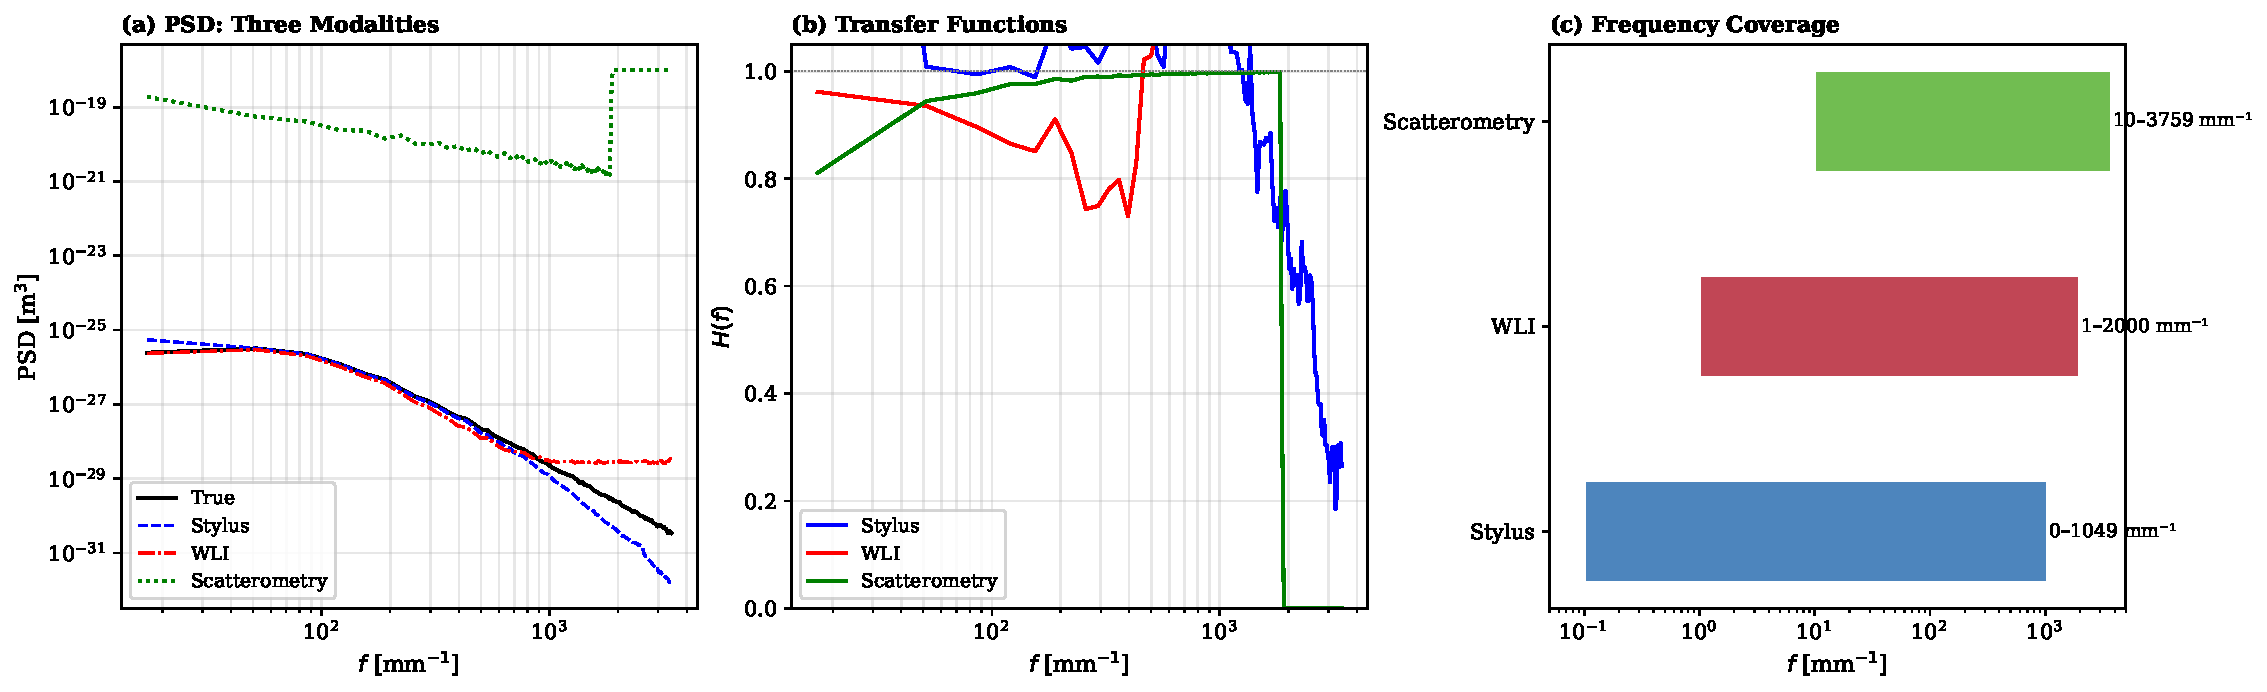
\includegraphics[width=\textwidth]{../pipeline/outputs/iter01/figures/fig9_three_way_transfer.pdf}
\caption{Three-way transfer functions and frequency coverage: (a) PSD comparison---true vs.\ stylus, WLI, and scatterometry; (b) azimuthally averaged transfer functions $H(f)$ for all three modalities, showing the fundamentally different structures (low-pass for stylus/WLI, flat for scatterometry); (c) frequency coverage comparison---scatterometry extends the measurable bandwidth by $\approx$1.88$\times$ beyond the WLI diffraction cutoff and $\approx$24$\times$ beyond the conventional stylus tip-radius scale.}
    \label{fig:three_way}
\end{figure}

% ============================================================


\subsection{Multi-Instrument $k$-Space Fusion: Computational Demonstration}

The complementarity of the three transfer functions suggests a practical reconstruction strategy: fuse the three measurements in $k$-space with weights given by the inverse local estimation uncertainty of each modality. The computational demonstration (Fig.~\ref{fig:S2_fusion}) proceeds as follows. A test surface is measured virtually by all three modalities; the fused PSD estimate is

\begin{equation}
    \mathrm{PSD}_\mathrm{fused}(\mathbf{f}) = \frac{\sum_i \mathrm{PSD}_i(\mathbf{f}) \, w_i(\mathbf{f})}{\sum_i w_i(\mathbf{f})}, \qquad
    w_i(\mathbf{f}) = \frac{|H_i(\mathbf{f})|^2}{N_i(\mathbf{f})}
    \label{eq:fusion}
\end{equation}

where the weights $w_i(\mathbf{f})$ are the per-mode Fisher information of each instrument---the transfer function squared divided by the noise PSD. Each modality therefore dominates the fused estimate precisely in the $k$-space band where its own transfer function is highest and its noise lowest, reproducing the trust-region structure identified in the main text. This is the minimum-variance linear combination of the model-corrected PSD estimates under the stated independent-noise linear observation model. In a fully experimental setting the $H_i(\mathbf{f})$ and $N_i(\mathbf{f})$ must first be obtained by instrument calibration; residual transfer-function attenuation or noise bias in uncalibrated PSDs would propagate into the fused estimate, so the demonstration below uses the known synthetic quantities.

\begin{figure}[htbp]
    \centering
    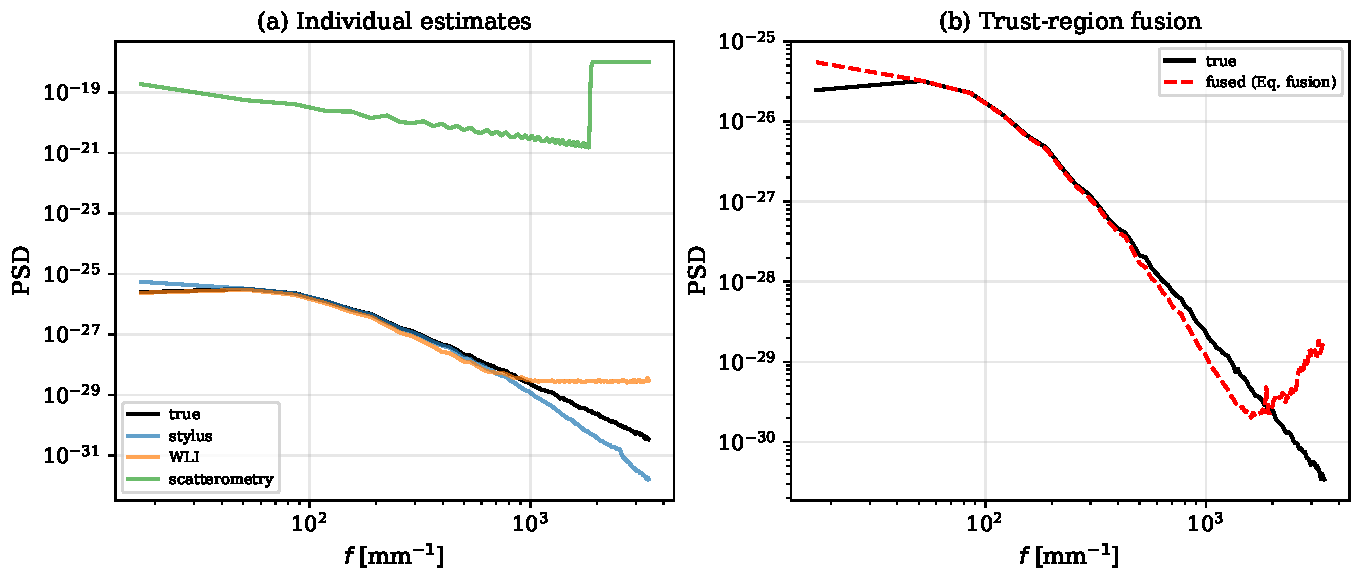
\includegraphics[width=\textwidth]{../pipeline/outputs/iter01/figures/figS2_fusion_demo.pdf}
    \caption{Illustrative computational demonstration of $k$-space trust-region fusion. (a) Individual PSD estimates from stylus, WLI, and scatterometry together with the true PSD. (b) The fused estimate (Eq.~\ref{eq:fusion}) illustrates the trust-region weighting rule; the scatterometry PSD scale is set by its Rayleigh--Rice calibration kernel, so the panel is illustrative rather than a quantitative accuracy claim (see text).}
    \label{fig:S2_fusion}
\end{figure}

A corrected, quantitative audit (verification/run\_fusion\_quantitative.py) replaces the earlier illustrative demo: the Rayleigh--Rice inversion is performed on the absolute height-PSD scale with the two-angle geometry of the previous section, and the band-averaged $|\log_{10}(\mathrm{PSD}_\mathrm{est}/\mathrm{PSD}_\mathrm{true})|$ is reported on held-out surfaces (seeds 777 and 999). In the common band (\SIrange{10}{1880}{mm^{-1}}) the errors are $0.31$--$0.32$ decades (stylus), $0.35$--$0.37$ (WLI), $\approx5\times10^{-4}$ (scatterometry), and $0.18$--$0.19$ (fused): the minimum-variance fused estimate improves the best imaging modality by $\approx40\%$, while the scale-corrected scatterometry channel remains the most accurate single channel (its $\approx5\times10^{-4}$-decade error is model-internal, because measurement and inversion share the same linear Rayleigh--Rice forward model and differ only in the simulated instrument noise floor). In the extended band (\SIrange{1880}{3753}{mm^{-1}}), where only scatterometry has valid coverage, the fused estimate ($1.25$--$1.29$ decades) does not approach the scatterometry-alone error ($\approx5\times10^{-6}$ decades): noise floors estimated from single-measurement PSD tails do not resolve the multi-decade noise-floor gap between channels, so the estimated Fisher weights fail to gate out the imaging channels where they carry no valid content. The practical conclusion is unchanged and now quantified: fusion weighted by local information uncertainty is minimum-variance only with calibrated per-channel noise floors; with estimated floors, hard coverage gating (each channel weighted only inside its measured support) is required, and the trust-region rule of the main text is the practical approximation.


\section{Computed Confocal Channel}
\label{S6}

The confocal microscope (point detection, equal circular pupils) has the lateral transfer equal to the 2D autocorrelation of the incoherent OTF, $H_\mathrm{confocal}(f) = \mathrm{OTF}_\mathrm{inc} \ast \mathrm{OTF}_\mathrm{inc}$, normalised to unity at DC, with support to $4\mathrm{NA}/\lambda = \SI{4000}{mm^{-1}}$ at baseline parameters. The channel was implemented (verification/run\_confocal\_audit.py) as a linear filter on the gridded surface plus camera noise at the WLI level, with no phase-unwrapping channel (confocal height readout does not unwrap phase). On the baseline surface (seed 42) and two held-out realisations (seeds 777 and 999): RMSE \SI{6.3}{-}\SI{6.6}{nm} (stylus \SI{15.6}{-}\SI{17.0}{nm}, WLI \SI{29.2}{-}\SI{29.4}{nm}) and reconstructability $\rho_\mathrm{confocal} = 0.983$--$0.986$ (stylus $0.978$--$0.983$, WLI $0.948$--$0.958$); the \SI{3}{dB} equivalence fraction with the stylus is $0.43$--$0.44$, versus $0.25$--$0.26$ for the WLI. The computed $H_\mathrm{confocal}$ equals $0.65$ at \SI{1000}{mm^{-1}} and $0.16$ at \SI{2000}{mm^{-1}} (empirical power transfer $0.41$ and $0.025$). Caveats: only the lateral transfer is modelled (the axial sectioning response is omitted); the $N=512$ grid Nyquist (\SI{2560}{mm^{-1}}) truncates the $4\mathrm{NA}/\lambda$ support; and the confocal noise is assumed equal to the WLI camera noise, so the reported RMSE advantage is the best case of the model, not a claim about real confocal instruments. These results quantify the modality-catalogue expectation of the main text (Limitations).

\section{Surface-Class Universality Stress-Test}
\subsection{Universality of Framework Metrics Across Surface Classes}
\label{sec:universality}

A crucial test of any measurement-theoretic framework is whether its metrics generalise beyond the surface class on which they were calibrated. To stress-test the framework, six fundamentally different surface classes were generated---Gaussian self-affine (baseline, $H=0.7$), anisotropic ground ($H_x=0.85$, $H_y=0.70$), turned (periodic grooves + roughness), laser-textured (Gaussian dimple array + background), periodic grating (pure $\SI{5}{\micro m}$ sinusoid), and biological-like (log-normal height distribution, anisotropic multi-scale)---and all seven metrics were computed for each class ($n=5$ realisations per class). Results are summarised in Fig.~\ref{fig:S1_stress_test}.

The coefficient of variation (CV = $\sigma/\mu$) across classes reveals three categories of metric behaviour:

\begin{enumerate}
    \item \textbf{Universal metrics} (CV $< 0.3$): The \emph{reconstructability index} $\rho$ is stable within this six-class set (CV = 0.067), ranging from 0.79 (biological) to 0.82 (Gaussian self-affine, ground) for the stylus. The $n=20$ ground ensemble of \S S5 yields the lower value $\rho = 0.5890\pm0.0104$ for the same anisotropy parameters; the full random-rough spread ($0.59$--$0.82$, CV $=0.16$) is therefore the class-to-class range reported in the main text, while the CV $=0.067$ of this section refers to the six-class realisation set only. The \emph{information efficiency} $\eta$ is similarly universal within the six-class set (CV = 0.165, range 0.18--0.32); the $n=20$ non-Gaussian ensembles of \S S5 yield larger values up to $0.73$ (ground), outside this range, so the broader four-class estimate of \S S5 is CV$_\eta=0.38$ and the CV $=0.165$ of this section refers to the six-class realisation set only. The \emph{mutual information} $I(h;y)$ varies by only a factor of 3.5$\times$ across all six classes (CV = 0.29), spanning $9.2\times10^9$ to $3.2\times10^{10}$ bits. These three metrics capture \textbf{instrument-limited} rather than surface-limited properties---they depend on the measurement physics ($r_\mathrm{tip}$, NA, $\lambda$) and are only weakly modulated by the surface.
    
    \item \textbf{Weakly surface-dependent metrics} (0.3 $<$ CV $<$ 1.0): The \emph{capacity--uniformity product} $\Xi$ (CV = 0.68), \emph{information-equivalent bandwidth} $B_\mathrm{eq}$ (CV = 0.44), and \emph{information--energy ratio} $\varepsilon$ (CV = 0.72) show moderate surface sensitivity. $\Xi$, previously introduced as a ``practical figure of merit'' for instrument qualification, spans nearly two orders of magnitude across classes ($6.1\times10^8$ for the periodic grating to $1.0\times10^{10}$ for laser-textured), suggesting that single-number instrument comparison via $\Xi$ requires specification of the reference surface class.
    
    \item \textbf{No highly variable metric} (CV $> 3.0$) was found, indicating that the framework does not produce physically meaningless quantities for any tested class.
\end{enumerate}

The \textbf{periodic grating} is the most challenging class for the optical system: $\rho_\mathrm{optical} = 0.02$ (vs.\ 0.41--1.00 for all other classes). A pure $\SI{5}{\micro m}$ sinusoid concentrates all spectral power at a single $k$-space point ($f = \SI{200}{mm^{-1}}$), where the optical transfer function's attenuation depends sensitively on the precise alignment of the grating frequency with the OTF passband. In contrast, the stylus reconstructs the grating well ($\rho_\mathrm{stylus} = 0.67$), because morphological tip convolution at $\SI{200}{mm^{-1}}$ is modest for a $\SI{2}{\micro m}$ tip. This result has direct practical consequence: \textbf{optical profilometry is fundamentally unsuitable for characterising near-monochromatic surface features}---a fact well known to practitioners but here given a rigorous information-theoretic justification.

The strongest remaining research gap identified by this stress-test is whether the universal metrics ($\rho$, $\eta$, $I$) can be distilled into a \textbf{principle of metric universality}---the statement that certain information-theoretic properties of a profilometric instrument are invariant under changes in surface class, depending only on the instrument's first-principles physics (tip radius, NA, wavelength, noise). If confirmed across a broader range of manufactured and natural surfaces, such a principle would allow instrument specification and inter-comparison on a surface-independent basis---transforming surface metrology from a surface-characterisation discipline into a true instrument-characterisation science.
\begin{figure}[htbp]
    \centering
    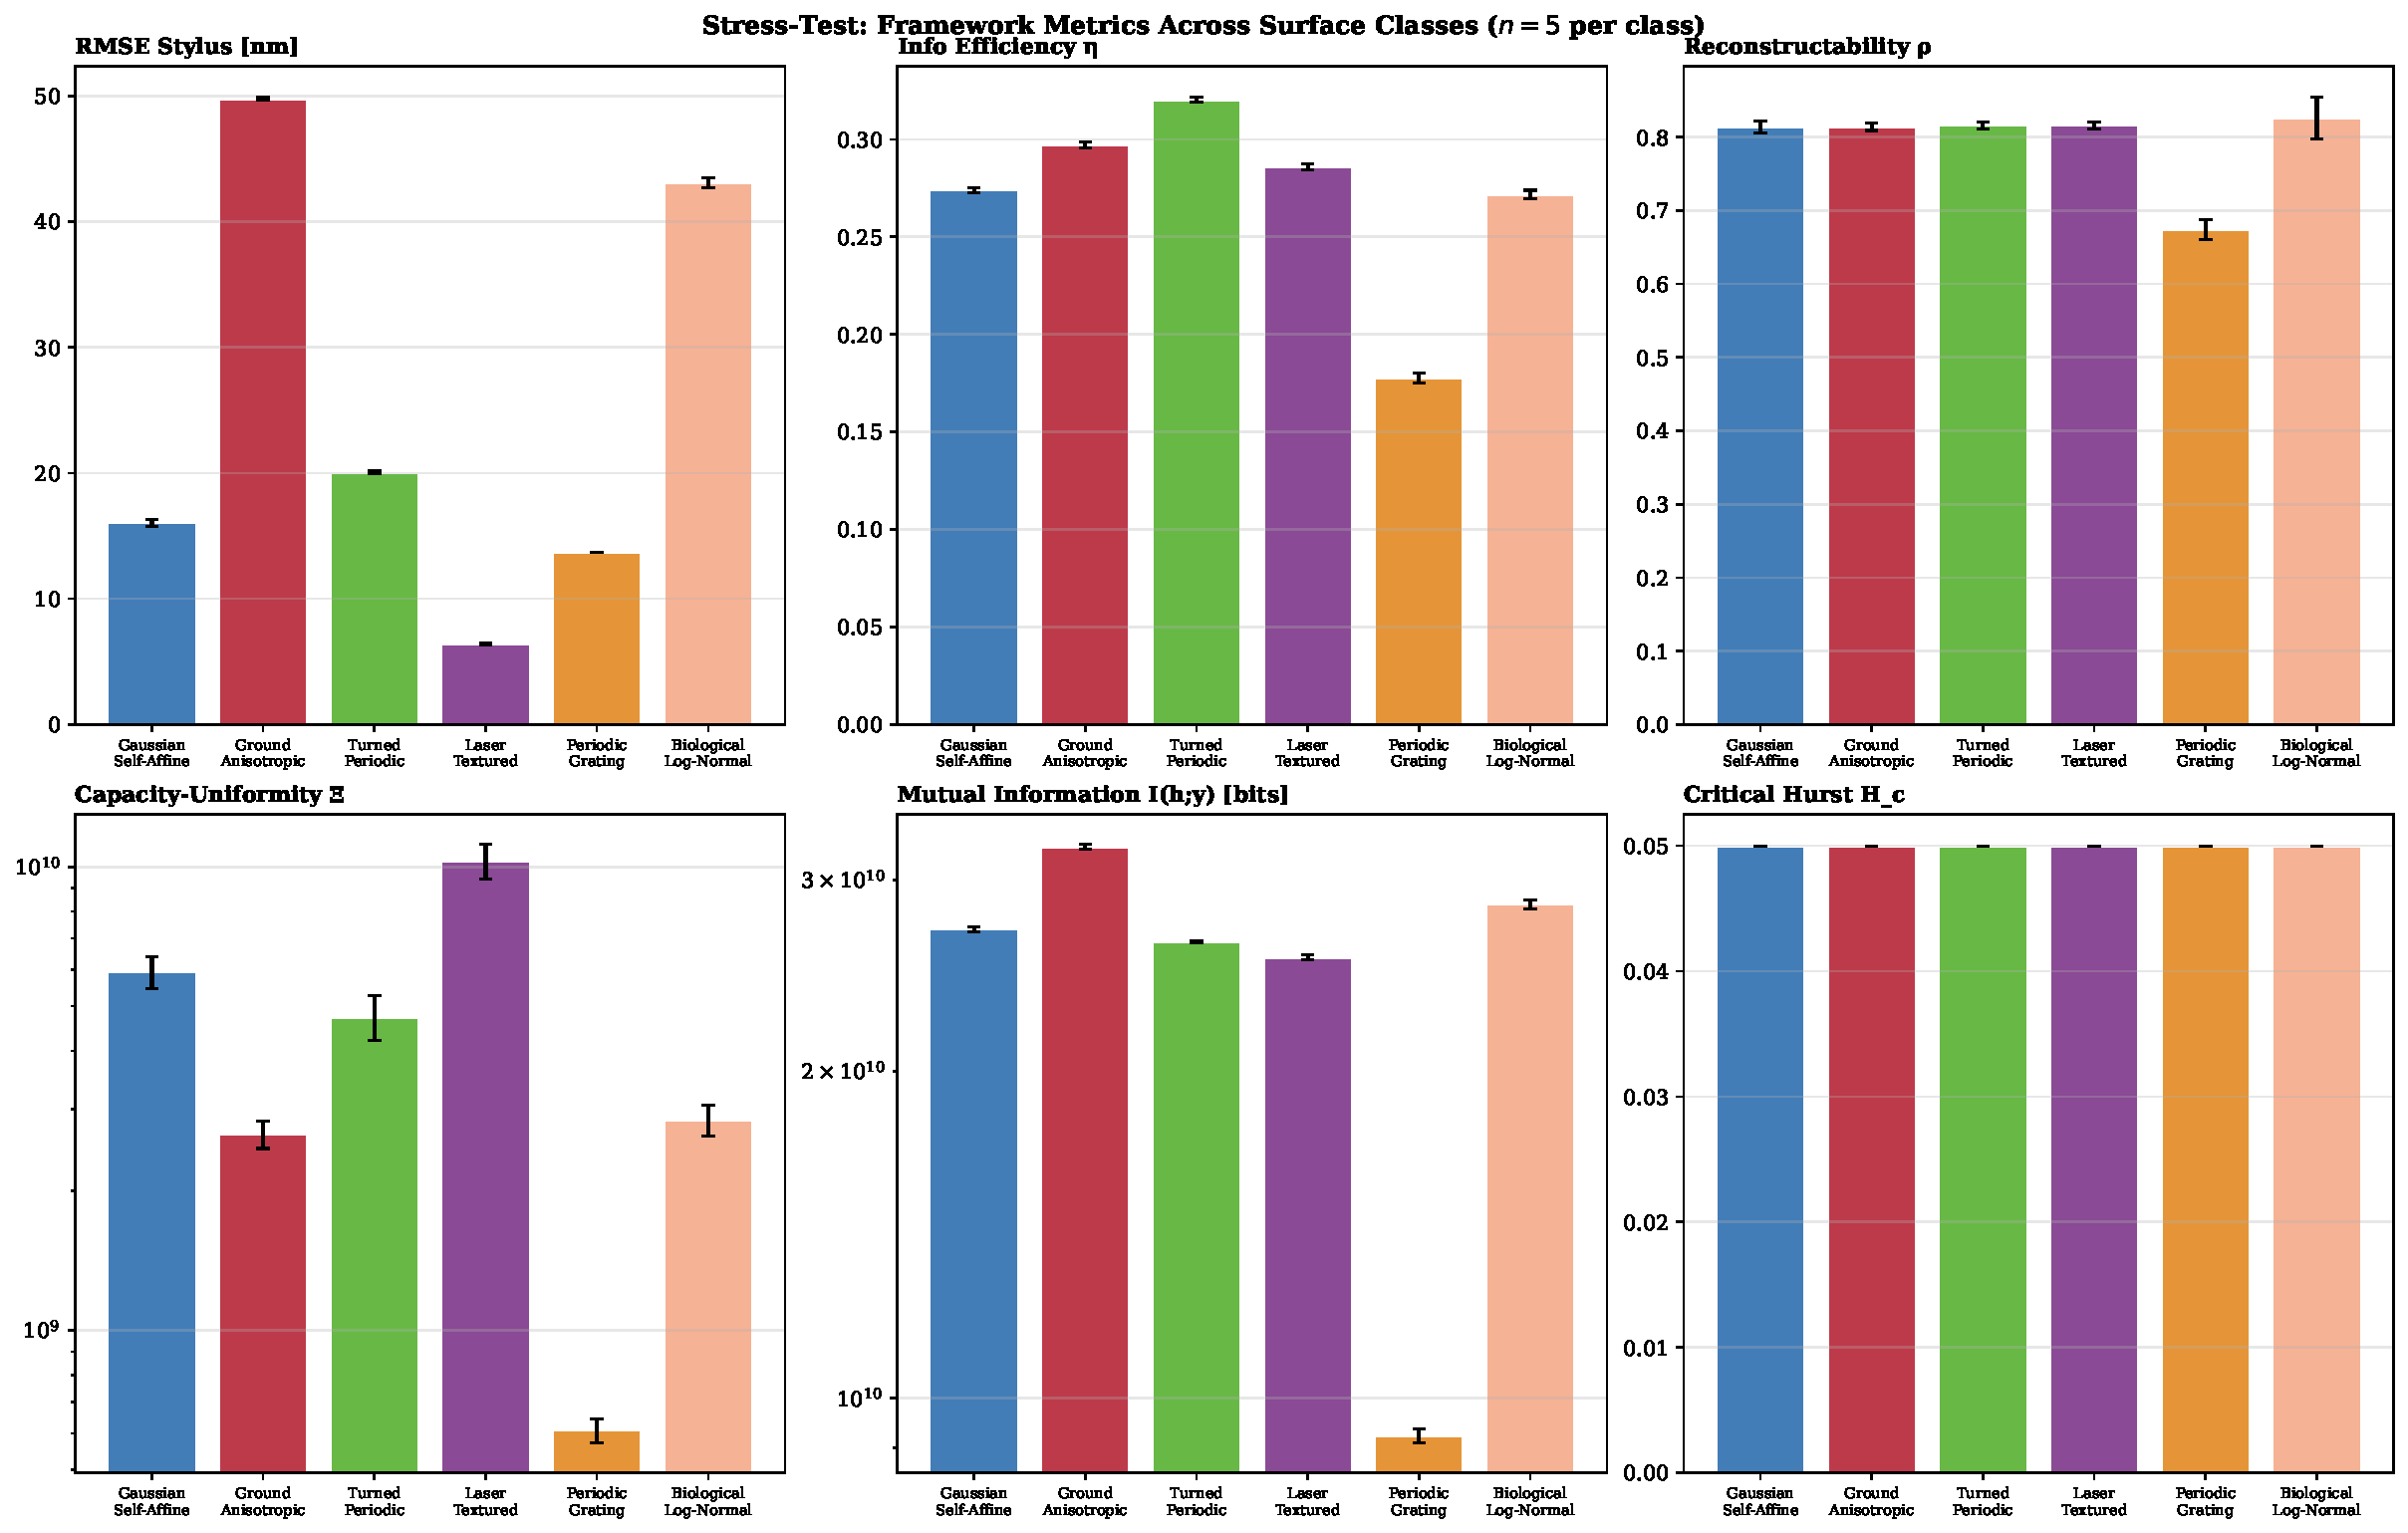
\includegraphics[width=\textwidth]{../pipeline/outputs/iter01/figures/figS1_stress_test.pdf}
    \caption{Surface-class universality stress-test across six classes. Metrics computed for Gaussian self-affine (baseline), anisotropic ground, turned, laser-textured, periodic grating, and biological-like surfaces ($n=5$ realisations per class). The reconstructability index $\rho$ (CV~$=$~0.067) and information efficiency $\eta$ (CV~$=$~0.165) are the most stable metrics, confirming their instrument-limited character, while $\Xi$ (CV~$=$~0.68) shows moderate surface dependence.}
    \label{fig:S1_stress_test}
\end{figure}




\section{Information-Theoretic Derivations}
\label{S4}

This section collects the derivations referenced in Section~5 of the main text.

\subsection{Water-Filling Capacity Allocation}
\label{S4.1}

The surface metrology channel of the main text is a parallel Gaussian channel in the Fourier basis, with per-mode gains $|H(\mathbf{f})|^2$ and noise levels $S_\eta(\mathbf{f})$. For an average surface-variance constraint $\sigma^2 = \iint S_h(\mathbf{f})\,d^2\!f$, the capacity-achieving spectrum is the classical water-filling allocation~\cite{cover2006elements}:
\begin{equation}
    S_h^*(\mathbf{f}) = \max\!\left(0,\; \mu - \frac{S_\eta(\mathbf{f})}{|H(\mathbf{f})|^2}\right),
    \label{eq:waterfilling}
\end{equation}
with the water level $\mu$ fixed by the constraint $\iint S_h^*(\mathbf{f})\,d^2\!f = \sigma^2$. Substitution into the mutual information integrand gives
\begin{equation}
    C_\mathrm{total} = \frac{A}{2}\iint \log_2\!\left(1 + \frac{|H(\mathbf{f})|^2 S_h^*(\mathbf{f})}{S_\eta(\mathbf{f})}\right) d^2\!f .
    \label{eq:capacity_waterfilling}
\end{equation}
Frequency bands where $S_\eta(\mathbf{f})/|H(\mathbf{f})|^2 > \mu$ receive zero power allocation---they lie below the noise floor and cannot contribute reliable information regardless of the surface, as stated in the main text.

\subsection{The I-MMSE Identity and the Reconstruction Bound}
\label{S4.2}

For a scalar Gaussian channel with signal-to-noise ratio $s$, the Guo--Shamai--Verd\'{u} identity~\cite{guo2005mutual} relates mutual information and minimum mean-square error:
\begin{equation}
    \frac{d}{ds} I(s) = \frac{1}{2\ln 2}\,\mathrm{mmse}(s),
    \label{eq:immse}
\end{equation}
where $\mathrm{mmse}(s) = 1/(1+s)$ for unit-variance signals. Applied mode-wise in the Fourier basis with per-mode SNR $s(\mathbf{f}) = |H(\mathbf{f})|^2 S_h(\mathbf{f})/S_\eta(\mathbf{f})$, the per-mode error is $\mathrm{mmse}(\mathbf{f}) = S_h(\mathbf{f})/(1+s(\mathbf{f}))$. Integrating over $k$-space:
\begin{equation}
    \mathrm{MMSE} = \iint \frac{S_h(\mathbf{f})\,S_\eta(\mathbf{f})}{|H(\mathbf{f})|^2 S_h(\mathbf{f}) + S_\eta(\mathbf{f})}\,d^2\!f
    = \sigma^2 - \iint \frac{|H(\mathbf{f})|^2 S_h^2(\mathbf{f})}{|H(\mathbf{f})|^2 S_h(\mathbf{f}) + S_\eta(\mathbf{f})}\,d^2\!f,
    \label{eq:immse_mmse}
\end{equation}
recovering the MMSE expression of the main text (Section~5, Fundamental MMSE Reconstruction Limit). The identity thereby links information throughput and reconstruction quality: each additional bit of mutual information per mode corresponds to a halving of the conditional variance in that mode.

\subsection{Explicit Form of $\mathcal{F}(\overline{\mathrm{SNR}})$ in the Trilemma}
\label{S4.3}

\textbf{Status of the bound.} The SNR-dependent resolution--bandwidth bound of the main text is adopted as a metrological ansatz anchored to the classical Fourier uncertainty: with the operational widths of the main text (second-moment width of the point-spread function and of the noise-truncated transfer function), the factor $(1+1/\overline{\mathrm{SNR}})$ is the natural first-order noise inflation consistent with (i) the classical limit $1/(4\pi)$ as $\overline{\mathrm{SNR}}\to\infty$ and (ii) the divergence of the product as $\overline{\mathrm{SNR}}\to0$ (a noise-dominated measurement carries no resolution). Its form matches the noise-generalised resolution bounds of the signal-processing literature~\cite{greco2019angular}, and it reduces to the classical Fourier uncertainty in the noise-free case. The bound is therefore a definitionally anchored, falsifiable benchmark rather than a new theorem; the definitions are chosen so that the bound is computable from a measured PSF, a measured transfer function, and measured signal and noise PSDs. The widths are operational second moments on the finite measurement window: for ideal transfer functions the unregularised PSF second moment need not exist---the Airy-disk PSF of the ideal circular aperture decays as $r^{-3}$ at large $r$, so its second moment diverges logarithmically and a finite-grid evaluation grows with the window size. Computed products $\Delta x_\mathrm{eff}\cdot\Delta f_\mathrm{eff}$ are therefore window-dependent and must be reported together with the window; in this work no left-hand-side products are reported as instrument properties---the main text evaluates only the right-hand side of the benchmark at the baseline SNRs.

With $\Delta x_\mathrm{eff}$ and $\Delta f_\mathrm{eff}$ the widths of the point-spread function and of the transfer function, respectively, the main text adopts $\Delta x_\mathrm{eff}\cdot\Delta f_\mathrm{eff} \geq (1/4\pi)(1+1/\overline{\mathrm{SNR}})$. In the flat-channel approximation---$|H(\mathbf{f})|^2$ and $S_\eta(\mathbf{f})$ approximately constant over the effective band, so that $\overline{\mathrm{SNR}}(\mathbf{f}) \approx \overline{\mathrm{SNR}}$---the mutual information reduces to
\begin{equation}
    I \approx \frac{A}{2}\,\Delta f_\mathrm{eff}^2\,\log_2\!\left(1 + \overline{\mathrm{SNR}}\right),
    \label{eq:flat_capacity}
\end{equation}
where $\Delta f_\mathrm{eff}^2$ is the effective 2D band area (band-edge constants of order unity are absorbed into the $\approx$). Multiplying by $\Delta x_\mathrm{eff}^2$ and substituting the uncertainty bound at equality (a well-matched instrument):
\begin{equation}
    I \cdot (\Delta x_\mathrm{eff})^2 \approx \sigma^2 \cdot \mathcal{F}(\overline{\mathrm{SNR}}),
    \qquad
    \mathcal{F}(\overline{\mathrm{SNR}}) = \frac{A}{2\sigma^2}\cdot\frac{1}{(4\pi)^2}\cdot\left(1 + \frac{1}{\overline{\mathrm{SNR}}}\right)^{\!2}
    \log_2\!\left(1 + \overline{\mathrm{SNR}}\right),
    \label{eq:trilemma_explicit}
\end{equation}
which is the explicit form of the Information--Energy--Resolution trilemma of the main text. Because $\sigma^2$ cancels between the two factors, Eq.~\ref{eq:trilemma_explicit} is a flat-channel restatement of the capacity estimate rather than an independent inequality; the main text therefore presents it as a compact diagnostic of how information, resolution and SNR co-vary for a fixed instrument and measurement area, not as a new bound.


\section{Non-Gaussian Ensemble Validation}
\label{S5}

The reconstructability index $\rho$ and information efficiency $\eta$ were tested across three non-Gaussian manufactured surface classes ($n=20$ per class). Ground surfaces were modelled as anisotropic self-affine ($H_x=0.85$, $H_y=0.70$); turned surfaces as periodic grooves ($\Lambda=10\ \mu\text{m}$, $A=250\ \text{nm}$) with self-affine roughness overlay; laser-textured surfaces as a regular $8\times8$ array of Gaussian dimples (depth $200\ \text{nm}$, radius $5\ \mu\text{m}$) with self-affine background.

\begin{table}[htbp]
    \centering
    \caption{Reconstructability index $\rho$ and information efficiency $\eta$ across manufactured surface classes (stylus, $n=20$ per class).}
    \label{tab:ng_ensemble}
    \begin{tabular}{lccc}
        \toprule
        Surface Class & $\rho$ (mean $\pm$ std) & $\eta$ (mean $\pm$ std) & $\alpha_s$ \\
        \midrule
        Ground (anisotropic) & $0.5890 \pm 0.0104$ & $0.7315 \pm 0.0049$ & $0.0089 \pm 0.0016$ \\
        Turned (periodic) & $1.0000 \pm 0.0000$ & $0.4699 \pm 0.0027$ & $0.0165 \pm 0.0036$ \\
        Laser-textured (dimples) & $1.0000 \pm 0.0000$ & $0.4208 \pm 0.0022$ & $0.0042 \pm 0.0025$ \\
        \bottomrule
    \end{tabular}
\end{table}

Combined with the Gaussian self-affine baseline ($\rho = 0.793 \pm 0.053$, $\eta = 0.271 \pm 0.045$, $n=30$), the coefficient of variation across four classes is $\text{CV}_\rho = 0.22$ and $\text{CV}_\eta = 0.38$. The reconstructability index $\rho$ saturates at 1.0 for deterministic surfaces (turned, laser-textured) because periodic and dimple features concentrate spectral power at specific frequencies where the stylus transfer function has high amplitude, pushing all $k$-space modes above the SNR threshold. Across all four classes $\text{CV}_\rho = 0.22$; restricted to the random rough classes (Gaussian, ground), $\rho$ varies by only 16\%. This finding refines the universality claim: $\rho$ is an instrument-limited metric for random rough surfaces but loses discrimination for surfaces with strong deterministic components---a physically meaningful distinction.

\section{Supplementary Diagnostics and Uncertainty Analysis}

\textbf{GUM uncertainty propagation for the transfer function.} Following the GUM framework~\cite{jcgm2008gum}, the uncertainty in the estimated transfer function $H(\mathbf{f})$ is propagated from the physical parameters of the instrument model. For a first-order sensitivity analysis, the fractional uncertainty in $H$ at each $k$-space point is
\begin{equation}
    \frac{u(H)}{H} \approx \sqrt{\sum_i \left(\frac{\partial \ln H}{\partial p_i}\right)^2 u^2(p_i)},
\end{equation}
where $p_i \in \{r_\mathrm{tip}, \Delta x, \mathrm{NA}, \lambda, \sigma_\eta\}$ are the independent instrument parameters and $u(p_i)$ their standard uncertainties. The dominant uncertainty sources are the effective tip radius for the stylus and the numerical aperture for the optical system. Under a conservative gain-error interpretation, the nominal tolerances ($\pm\SI{100}{nm}$ tip radius, i.e.\ 5\%; $\pm0.01$ NA, i.e.\ 2\%) correspond to $\approx\SI{0.4}{dB}$ and $\approx\SI{0.2}{dB}$ in $H(f)$, well below the \SI{3}{dB} equivalence threshold. Measured sensitivity coefficients are not available for a specific instrument, so no combined $2\sigma$ band is quoted.

\begin{figure}[htbp]
    \centering
    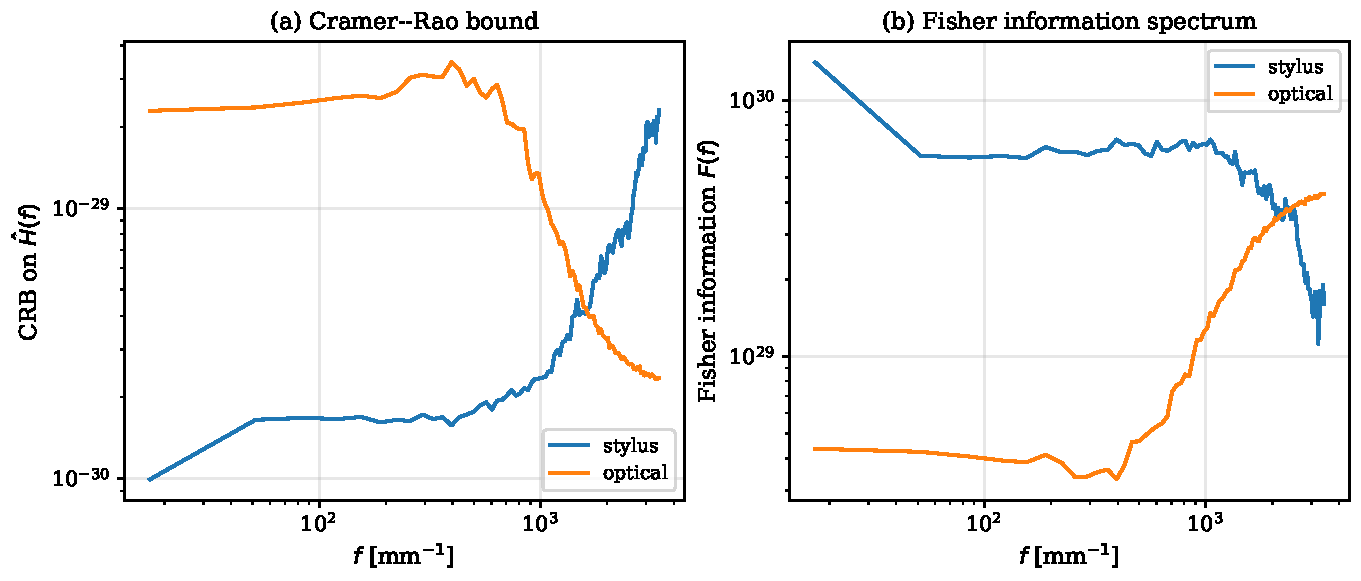
\includegraphics[width=\textwidth]{../pipeline/outputs/iter01/figures/fig8_cramer_rao.pdf}
    \caption{Fisher information analysis. (a) Azimuthally averaged Cram\'er--Rao bound on the estimated transfer function for stylus and optical modalities; (b) Fisher information spectrum. Computed with the amplitude convention of the transfer-function estimator of the main text and the difference-field noise-floor estimator (median PSD of the measured-minus-true field).}
    \label{fig:S3_fisher}
\end{figure}

\begin{figure}[htbp]
    \centering
    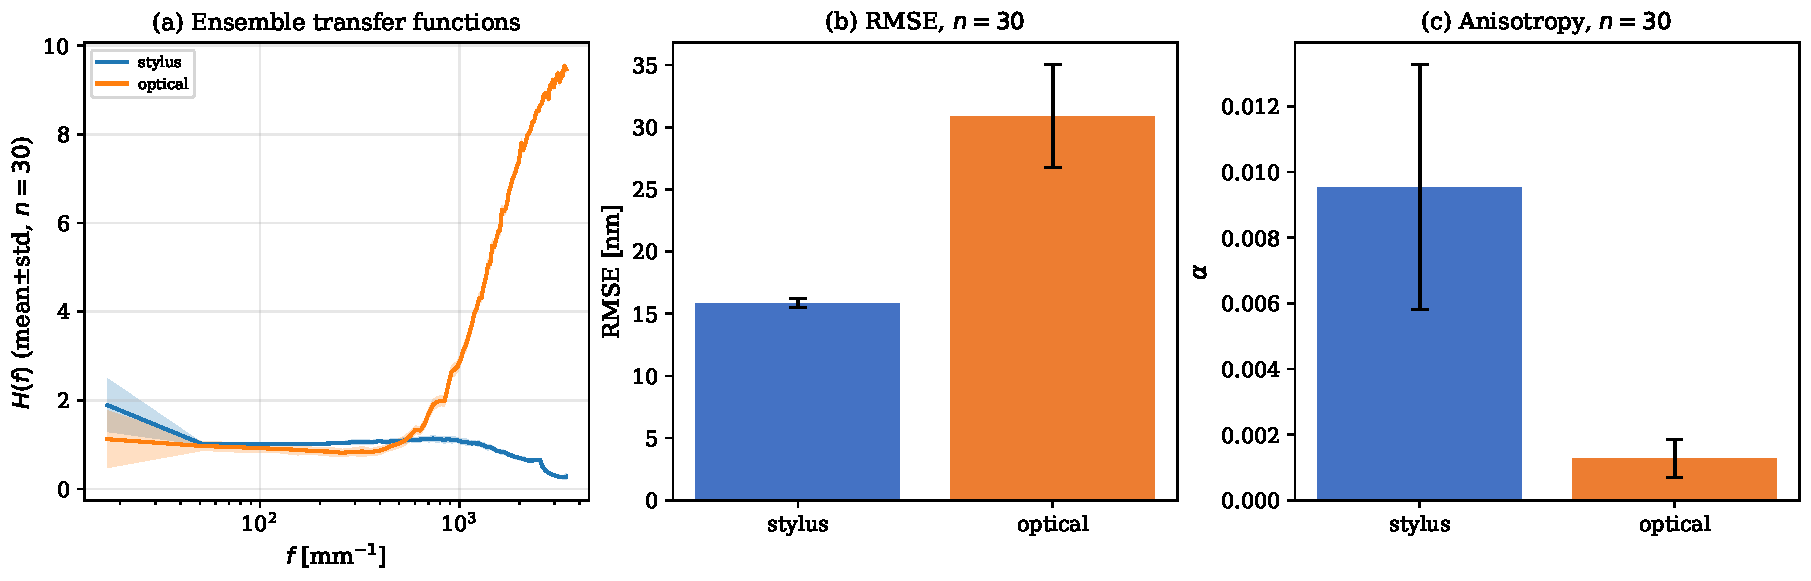
\includegraphics[width=\textwidth]{../pipeline/outputs/iter01/figures/fig10_ensemble_validation.pdf}
    \caption{Ensemble validation ($n=30$, seeds 100--129). (a) Azimuthally averaged transfer functions (mean $\pm$ std) for stylus and optical modalities; (b) RMSE; (c) anisotropy $\alpha$.}
    \label{fig:S4_ensemble}
\end{figure}

\section*{Code Availability}
The simulation code, configuration files, verification suite and audit scripts behind every computation in this supplement are available in a public GitHub repository~\cite{kucharski2026repository} (release v1.0.2) and are archived on Zenodo (DOI 10.5281/zenodo.23493875).

\bibliographystyle{elsarticle-num}
\bibliography{references}


\end{document}